\section{Introduction}

\subsection[Overview]{History of Cryptocurrency}
\vspace*{-0.5cm}

\begin{minipage}[h]{0.45\linewidth}
%Print version of table
\begin{warpprint}
\begin{table}[H]{}
\renewcommand\arraystretch{1.4}\arrayrulecolor{blue}
\captionsetup{singlelinecheck=false, labelfont=sc, labelsep=quad}
\caption{Timeline of Cryptocurrency}%\vskip -1.5ex
% lwarp table, and print edition (uncomment stuff below for good copy)
\begin{tabular}{c p{5cm}}%
% Good copy for print edition
%\begin{tabular}{@{\,}r <{\hskip 2pt} !{\foo} >{\raggedright\arraybackslash}p{5cm}}
%\toprule
%\addlinespace[1.5ex]
2008 & Bitcoin White Paper \\
2009 & Bitcoin Genesis Block\\
2013 & 1 BTC = \$ 31 USD\\
2013 & \gls{Ethereum} White Paper \\
2015 & \gls{Ethereum} Genesis Block\\
2015 & \gls{HyperLedger} starts \\
2017 & Over 1000 different cryptocurrencies \\
2018 & AWS Blockchain Templates \\
\end{tabular}
\end{table}
\end{warpprint}
% HTML VERSION OF TABLE
\begin{warpHTML}
\begin{table}[H]{}
\renewcommand\arraystretch{1.4}\arrayrulecolor{blue}
%\captionsetup{singlelinecheck=false, labelfont=sc, labelsep=quad}
\caption{Timeline of Cryptocurrency}%\vskip -1.5ex
% lwarp table, and print edition (uncomment stuff below for good copy)
\begin{tabular}{c p{5cm}}%
% Good copy for print edition
%\begin{tabular}{@{\,}r <{\hskip 2pt} !{\foo} >{\raggedright\arraybackslash}p{5cm}}
%\toprule
%\addlinespace[1.5ex]
2008 & Bitcoin White Paper \\
2009 & Bitcoin Genesis Block\\
2013 & 1 BTC = \$ 31 USD\\
2013 & \gls{Ethereum} White Paper \\
2015 & \gls{Ethereum} Genesis Block\\
2015 & \gls{HyperLedger} starts \\
2017 & Over 1000 different cryptocurrencies \\
2018 & AWS Blockchain Templates \\
\end{tabular}
\end{table}
\end{warpHTML}
\end{minipage}%
\begin{minipage}[h]{0.55\linewidth}
In 2008 bitcoin white paper \cite{bitcoinWhitePaper:Online} described a way to solve the double spending problem without a centralized body using \gls{blockchain}. Although, the value of bitcoin (BTC) has grown exponentially, high computational and energy consumption in mining and slow performance \cite{bitCoinProblems:Online}.  Released in July 30, 2015, Ethereum, an open-source platform based on blockchain technology, distinguishes itself from bitcoin through faster transactions, unlimited processing capability for \glspl{smart contract}, and its network is optimized to support \gls{DApp} \cite{ethereumWhitePaper:Online}.
\end{minipage}%
%\begin{figure}[ht]
%\begin{adjustbox}{center,max width=1.1\textwidth}
%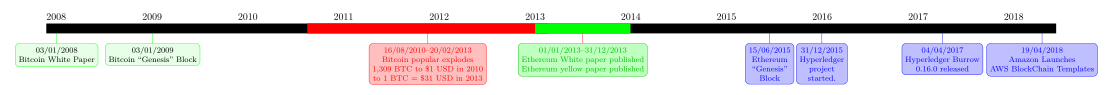
\includegraphics[width=1.2\linewidth]{Diagrams/advancedTimeline.pdf}
%\end{adjustbox}
%\caption{An example of server-blockchain architecture in a DAPP.}
%\label{fig:dappArc}
%\end{figure}



%%% Contain timeline
\vspace*{-0.25cm}
\subsection{Decentralized Applications}
%%% ClEAN TIHS UP LATER
	%A blockchain is a digitized, decentralized, public ledger of all cryptocurrency transactions. %To access websites on the Ethereum blockchain and use dapps a specialized browser is needed, or a browser plugin like \gls{MetaMask}. 
	Blockchain technology is revolutionizing the internet by establishing trust in shared data. \cite{book:bchainForDummies}.
	Additionally, transactions recorded on the blockchain are practically impossible to remove or change. 
	A decentralized application, or DApp are deployed on peer to peer networks such as Ethereum or on the cloud \footnotemark. A decentralized system (peer to peer) has many advantages over a conventional centralized network including no single points of failure, cheaper distribution (servers are expensive), faster upload speeds. 
	\footnotetext[1]{Amazon recently started offering blockchain templates on AWS. \cite{ethereumWhitePaper:Online}}
	
	\paragraph{Types of Blockchains}
	\begin{itemize}
	\item[---]  \textbf{Public blockchains} are large distributed networks that are run through a native token such as bitcoin or ether. Anyone can participate and the community maintains its open-source code. The two largest public blockchains are Ethereum and Bitcoin.%They’re open for anyone to participate at any level and have open-source code that their community maintains.
	% rewrite and add section about composer
	\item[---] \textbf{Permissioned blockchains} define role based access control for individuals in the network and uses native tokens.  \gls{HyperLedger Composer}, an open-source framework for permissioned blockchains, is used for smart contracts and for blockchain application development \cite{hyperledgerComposer:Online}. One use case is an accounting system that calculates payment, while hiding that information from unrelated organizations.  % Their core code may or may not be open source.
	\item[---] \textbf{Private blockchains}  membership is tightly controlled and lacks a native token. Useful for consortiums with trusted associates and exchanging confidential information, however, less powerful because it is supported by limited private resources.
	\end{itemize}
	\vspace*{-0.5cm}
	
	
	% Consider taking this part out, too detailed for the high level explaination.
	\paragraph{Public and Private Keys}
	 \textbf{In a blockchain} system, any key holder can use their private key to sign a piece of data. This results in a signature.  
	  In a Dapp, this can be used for:
	 \begin{enumerate}
		\item Recovering the public key (ethereum account address) of the Author.
		\item Verify if the raw data is the same as the one signed by Author using the public key. 
	\end{enumerate}
	
	%In order to sign something, a mathematical function is used to "sign" a piece of document/data. A digital signature of a document/data is a number generated using a private key. The private key has a corresponding public key. 
	
	
	
%	\begin{figure}[ht]
%	\centering
%	\includegraphics[width=0.5\linewidth]{Diagrams/verifySig.png}
%	\caption{Illustrate how public and private keys are used to verify signatures}
%	\label{fig:verfSig}
%	\end{figure}
	
		 
% refer to medium article, and some other article highlighting the interest in private nodes, https://aws.amazon.com/partners/blockchain/
% https://blog.zeppelin.solutions/designing-the-architecture-for-your-ethereum-application-9cec086f8317
% https://aws.amazon.com/blogs/apn/introducing-aws-blockchain-partners/

%		To access websites on the Ethereum blockchain and use dapps a specialized browser is needed, or a plugin like metamask. 

\subsection{Smart Contracts}
	\begin{warpprint}
	\begin{figure}[ht]
		\centering
		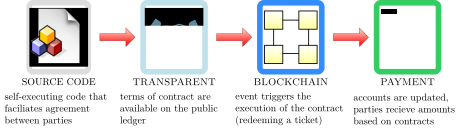
\includegraphics[width=1\linewidth]{Diagrams/smartContractsExp.pdf}
		\caption{Illustrating how a smart contract works}
		\label{fig:smartContracts}
	\end{figure}
	\end{warpprint}
	
	\begin{warpHTML}
	\begin{figure}[ht]
		\centering
		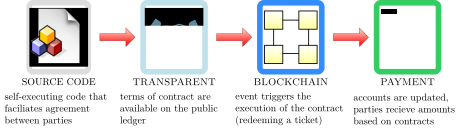
\includegraphics[width=1\linewidth]{Diagrams/smartContractsExp.svg}
		\caption{Illustrating how a smart contract works}
		\label{fig:smartContracts}
	\end{figure}
	\end{warpHTML}
	\newpage